\documentclass[12pt]{beamer}
%
% Choose how your presentation looks.
%
% For more themes, color themes and font themes, see:
% http://deic.uab.es/~iblanes/beamer_gallery/index_by_theme.html
%
\mode<presentation>

{
  \usetheme{PaloAlto}      % or try Darmstadt, Madrid, Warsaw, ...
  \usecolortheme{whale} % or try albatross, beaver, crane, ...
  \usefonttheme{default}  % or try serif, structurebold, ...
  \setbeamertemplate{navigation symbols}{}
  \setbeamertemplate{caption}[numbered]
} 
%remove navigation symbols at bottom
\setbeamertemplate{navigation symbols}{}
\setbeamertemplate{footline}[frame number]
\setbeamertemplate{footline}[text line] {

	\makebox[.7\paperwidth]{
		\insertframenumber  /\inserttotalframenumber
		\hfill
	%	\url{http://envirohack.herokuapp.com/}
	}

}

% add logo
\usepackage{pgf}
%coords are in relation to lower right corner
\logo{\pgfputat{\pgfxy(-1.6,7.6)}{\pgfbox[center,base]{
\includegraphics[width=2.5cm]{logo.png}}}}


%I had problems compiling doc on X230 without next two lines
\usepackage{etex}
\reserveinserts{28}
%On X530 it worked without problems

%\usepackage[utf8x]{inputenc}
%My std preamble for the docs
%\selectlanguage{british}%
\usepackage[british]{babel}
\usepackage{microtype} %better text
\IfFileExists{lmodern.sty}{\usepackage{lmodern}}{} %type 1 vector font
%
\usepackage{lettrine}
\usepackage{listings} %Add list support
\usepackage{colortbl} %colors in TABLES
%\usepackage{tikz,amsmath, amssymb,bm,color}
\usepackage{nicefrac}
\usepackage{lastpage} %get last page

%COLORS
\usepackage{color}
\definecolor{lightgray}{gray}{0.8} %for colortbl
\definecolor{UniBlue}{RGB}{83,121,170}
\definecolor{deepBlue}{HTML}{000066}
\definecolor{blueBgd}{HTML}{99C8FF}
\definecolor{aBlue}{HTML}{1879F7}

%%%%%%%%%%%%%%%%%%%%%%%%%%%%%%%%%%%%%%%%%%%%%%%%%%%%%%%%%%%%%%%%%%
%FOOTNOTES
%nice look after http://www.dedoimedo.com


%%%%%%%%%%%%%%%%%%%%%%%%%%%%%%%%%%%%%%%%%%%%%%%%%%%%%%%%%%%%%%%%%%%
%TABLE SETTINGS
\usepackage{colortbl} %colors in table
\usepackage{rotating} %rotatins within tables
\usepackage{multirow}
\renewcommand{\arraystretch}{1.2} %add padding/spacing
%\usepackage{adjustbox}%rotating and fitting into page
%

\usepackage{booktabs} % To thicken table lines
%define thickness of table lines
\let\mytoprule\toprule
\renewcommand{\toprule}{\mytoprule[0.20em]}
\let\mytoprule\bottomrule
\renewcommand{\bottomrule}{\mytoprule[0.20em]}
\let\mytoprule\midrule
\renewcommand{\midrule}{\mytoprule[0.08em]}

\usepackage{spreadtab} % for simple calculations

%vertically and horizontally centered multicolumn cells with a fixed width. M{width}
%\newcolumntype{M}[1]{>{\centering\hspace{0pt}}m{#1}}
% each spanned cell has the same width. S{width of multicolumn cell}{number of spanned columns}
%\newcolumntype{S}[2]{>{\centering\hspace{0pt}}m{(#1+(2\tabcolsep+\arrayrulewidth)*(1-#2))/#2}}

%%%%%%%%%%%%%%%%%%%%%%%%%%%%%%%%%%%%%%%%%%%%%%%%%%%%%%%%%%%%%%%%%%%
%TikZ
\usepackage{tikz}

\colorlet{red}{red!50}
\colorlet{green}{green!50}
\colorlet{blue}{blue!50}
\definecolor{yellow}{HTML}{FFFF00}
\colorlet{yellow}{yellow!50}
\definecolor{fiolet}{HTML}{7030A0}
\colorlet{fiolet}{fiolet!50}
\colorlet{bgd_main}{black!50}
\colorlet{bgd}{bgd_main!75}
\colorlet{bgd2}{bgd_main!50}
\colorlet{bgd3}{bgd_main!25}
\colorlet{bgd4}{bgd_main!15}

\usetikzlibrary{shapes,arrows,calc,positioning}

%%%%%%%%%%%%%%%%%%%%%%%%%%%%%%%%%%%%%%%%%%%%%%%%%%%%%%%%%%%%%%%%%%%
% Footnotes in Figs
%\rule[raise-height]{width}{thickness}
\newcommand*{\FigFootnote}[1]{
\noindent \begin{flushleft}
\rule[0.2ex]{0.4\columnwidth}{0.5pt}
\par
\footnotesize
#1
\footnotesize
\end{flushleft}
}

%%%%%%%%%%%%%%%%%%%%%%%%%%%%%%%%%%%%%%%%%%%%%%%%%%%%%%%%%%%%%%%%%%%
%MATH, number display
%need to install siunitx, l3kernel,l3packages
\usepackage{siunitx} %this is for units display

\sisetup{per-mode=fraction, tight-spacing = true , fraction-function = \nicefrac, quotient-mode = fraction}% %nicefrac \tfrac
\sisetup{inter-unit-product = \ensuremath { { } \cdot { } } , exponent-product = \cdot }%
\sisetup{input-product=x , output-quotient =  \ensuremath { { } \times{}}} %for 1x2x3
%number grouping(3), std==true %\sisetup{group-digits = decimal} 
\sisetup{group-minimum-digits = 4} %start grouping from 4 digits, in 3 no groups
\sisetup{range-units = single,range-phrase = \,--\,} %2-3C not 2C-3C %, range-phrase = --
\sisetup{separate-uncertainty=true} %2+-1 not 2(1)
\sisetup{prefixes-as-symbols=true } % , scientific-notation = engineering false for 10^-9 ect ect , exp in multiple of 3
\sisetup{range-phrase = \,-\, } % , refo of ranges
%\sisetup{zero-decimal-to-integer, round-mode = places,round-precision = 3}
%\sisetup{add-arc-degree-zero=true , add-arc-minute-zero=true ,add-arc-second-zero=true} %for angle settings

%This is to auto convert ns,ms,us to 10^-xx s
\DeclareSIUnit[scientific-notation = engineering, prefixes-as-symbols=false]{\psec}{\pico\second}
\DeclareSIUnit[scientific-notation = engineering, prefixes-as-symbols=false]{\nsec}{\nano\second} 
\DeclareSIUnit[scientific-notation = engineering, prefixes-as-symbols=false]{\usec}{\micro\second}
\DeclareSIUnit[scientific-notation = engineering, prefixes-as-symbols=false]{\msec}{\milli\second} 

%...AND SOME UNITS
\DeclareSIUnit\dBm{dBm}
\DeclareSIUnit\ppm{ppm} %{\num{1e-6}}%{ppm}
\DeclareSIUnit\yr{yr} %{{361}\day}<-nice nice
\DeclareSIUnit\cy{cycle} %phase cycle
\DeclareSIUnit\epoch{epoch} %GPS/LL epoch
\DeclareSIUnit\inch{"} %inch 
\DeclareSIUnit\wk{week} %week
\DeclareSIUnit\hr{hrs} %hours
\DeclareSIUnit\min{minute} %hours
\DeclareSIUnit\mile{mi}
\DeclareSIUnit\Mcps{Mcps}
\DeclareSIUnit\bit{bit}
\DeclareSIUnit\chip{chip length}
%Other units
\newcommand*{\GBP}[1]{$\SI{#1}[\textsterling]{}$}


%%%%%SHORTHANDS (Standard Sentences)
%\newcommand*{\Myrange}[3]{$\textrm{\SIrange{#1}{#2}{#3}}$}


%how much work per week
\newcommand*{\wkWrk}[1]{$\SI{#1}{\hr\per\wk}$}

%references
\newcommand*{\tabref}[1]{shown in table \ref{#1} on page \pageref{#1}\xspace}
\newcommand*{\vref}[1]{\ref{#1} on page \pageref{#1}\xspace}


%\renewcommand{\baselinestretch}{1.2} %line spacing
%{\setstretch{1.0}\color{blue} text bla bla } for section strech
\renewcommand{\footnotesize}{\scriptsize}
%\usepackage[demo]{graphicx}
\usepackage{caption}
%\usepackage{subcaption}

\title[EnviroHack]{H24VSP Project 3 - Introduction to PPP}
\author{Lukasz K Bonenberg}
\institute{NGI}
\date{\today}

\begin{document}
	

\begin{frame}
	\titlepage
\end{frame}

	% Uncomment these lines for an automatically generated outline.
	\begin{frame}{Outline}
	  \tableofcontents
	\end{frame}



\section{Introduction}

\begin{frame}{Introduction}
	In this project we will learn more Network RTK and PPP technique, usign Leica GS10 and maritime Veripos LD5 receiver with AsterRx chipset. The goal of the practical is to compare both method.
	
	\medskip
	The aim for this presentation is:
	\begin{itemize}
		\item Refresh your knowledge and understanding of PPP technology.
		\item Highlight differences between two methods. 
		\item Explain practicalities of using Veripos LD5 receiver.
	\end{itemize}
	

\end{frame}

\section{VERIPOS Services}

\begin{frame}{VERIPOS Services}
	There are three different VERIPOS services:

	\begin{itemize}
		\item \textbf{VERIPOS Standard} uses single frequency DGPS with 1-2 metre accuracy.
		\item \textbf{VERIPOS Standard Plus} uses dual-frequency DGPS with 1-2 metre accuracy. 
		\item \textbf{VERIPOS Ultra/APEX} uses global orbit \& clock correction and dual-frequency GPS/GLONASS observations for dm level accuracy.
	\end{itemize}
 All services provide coordinates in ITRF2008 and are using Inmarsat geostationary satellites 25E, 98W, 143.5E, AORE, AORW, IOR, POR to transmit corrections. 
\end{frame}

\begin{frame}{VERIPOS Standard}
	
	\begin{itemize}	
	\item Provides RTCM Type 1, 2 \& 3 messages.
	\item Normal accuracy: 1-2m. 
	\item Typical latency: 4 seconds.
	\item Single difference (DGPS) using GPS C/A code \& L1 carrier phase
	\end{itemize}	
	
\end{frame}

\begin{frame}{VERIPOS Standard Plus}
	Standard Plus is intended to combat symptoms of ionospheric activity on DGPS and predominantly to be used at lower latitudes. 
	\begin{itemize}	
		\item Provides RTCM Type 1, 3, 15 messages.
		\item Normal accuracy: 1-2m. 
		\item Typical latency: 4 seconds.
		\item Single difference (DGPS) using GPS C/A, P code \& L1, L2 carrier phase
	\end{itemize}	
\end{frame}	

\begin{frame}[plain]{VERIPOS Standard Plus}
	
	\begin{figure}
		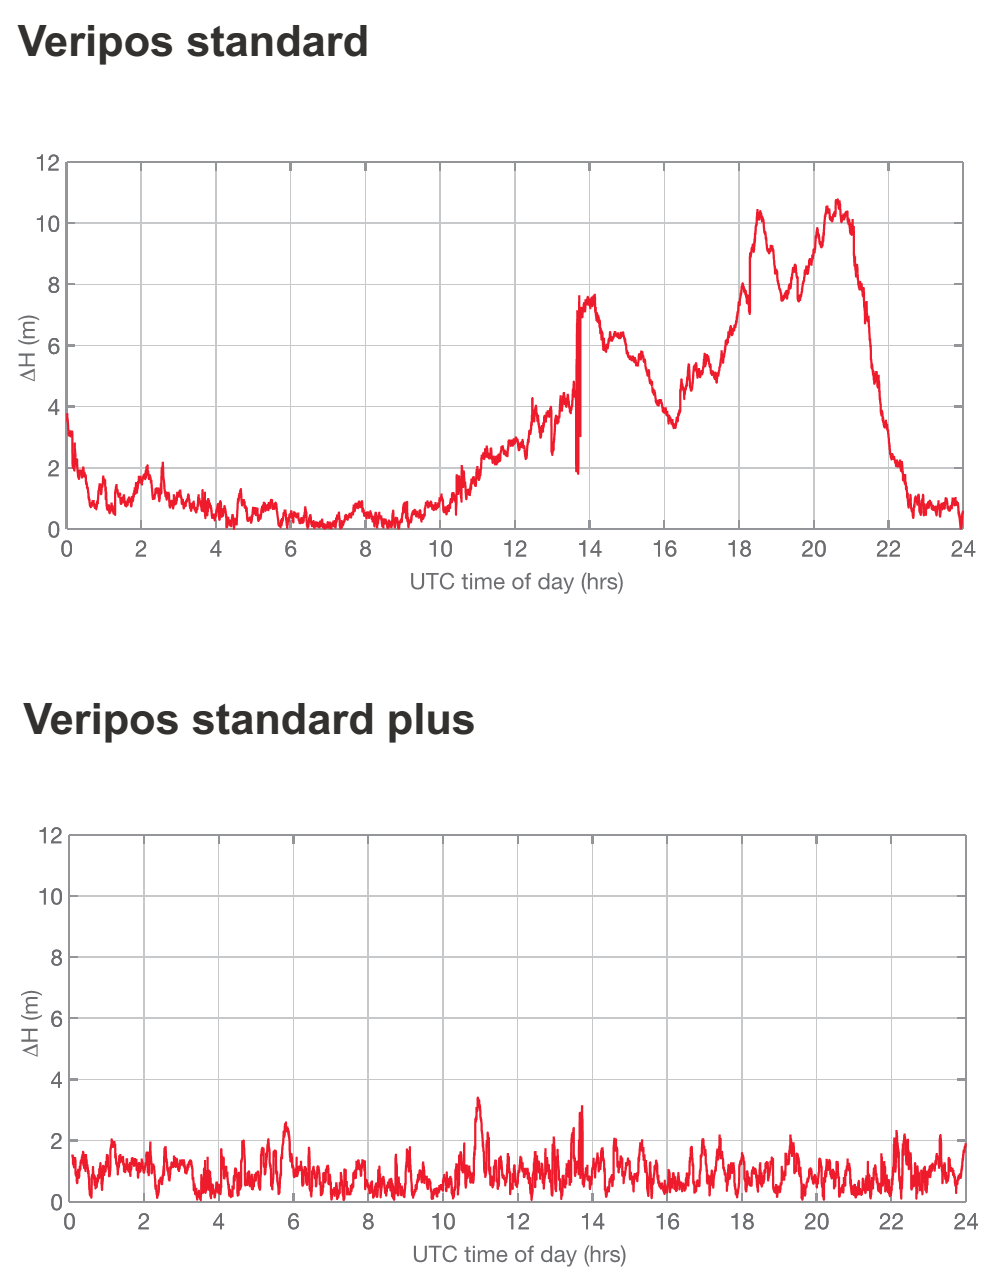
\includegraphics[height=0.9\textheight]{pic/StdPlus.png}
		%\caption{intro}
	\end{figure}

\end{frame}


\begin{frame}{VERIPOS Ultra}
 
	\begin{itemize}	
		\item Orbit and clock corrections in JPL GDGPS format
		\item Normal accuracy: 0.1m planar. 
		\item Typical latency: 2 seconds with 30 s update rate for clocks and 120s for orbits.
		\item Precise Point Positioning (PPP) using GPS L1/L2 carrier phase.
	\end{itemize}	
	
The reference station used in the Standard solution was located 322km distant at Kemaman.
\end{frame}	

\begin{frame}[plain]{VERIPOS Ultra}
	
	\begin{figure}
		
		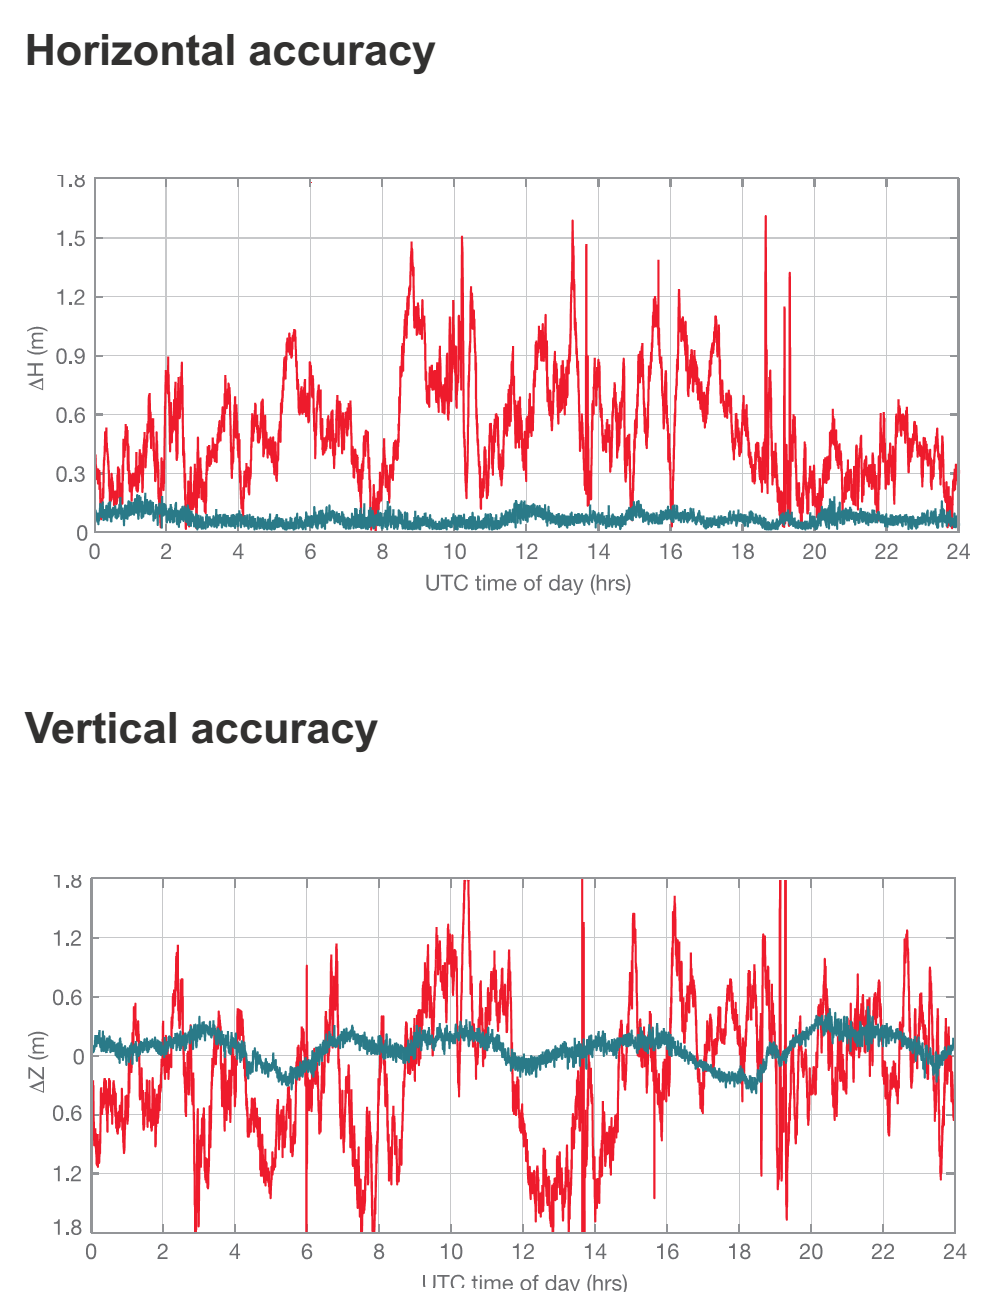
\includegraphics[height=0.8\textheight]{pic/Ultra.png}
		\caption{VERIPOS Standard and Ultra solutions at a monitor site in Singapore.}
	\end{figure}
	
\end{frame}

\begin{frame}{VERIPOS $Apex^2$}
	
	\begin{itemize}	
		\item Orbit and clock corrections in VERIPOS OCDS format
		\item Normal accuracy: 0.1m planar. 
		\item Typical latency: 2 seconds with 30 s update rate for clocks and 120s for orbits.
		\item Precise Point Positioning (PPP) using GPS and GLONASS L1/L2 carrier phase.
	\end{itemize}	


	
\end{frame}	


\begin{frame}[plain]{VERIPOS  $Apex^2$}
	
	\begin{figure}
		
		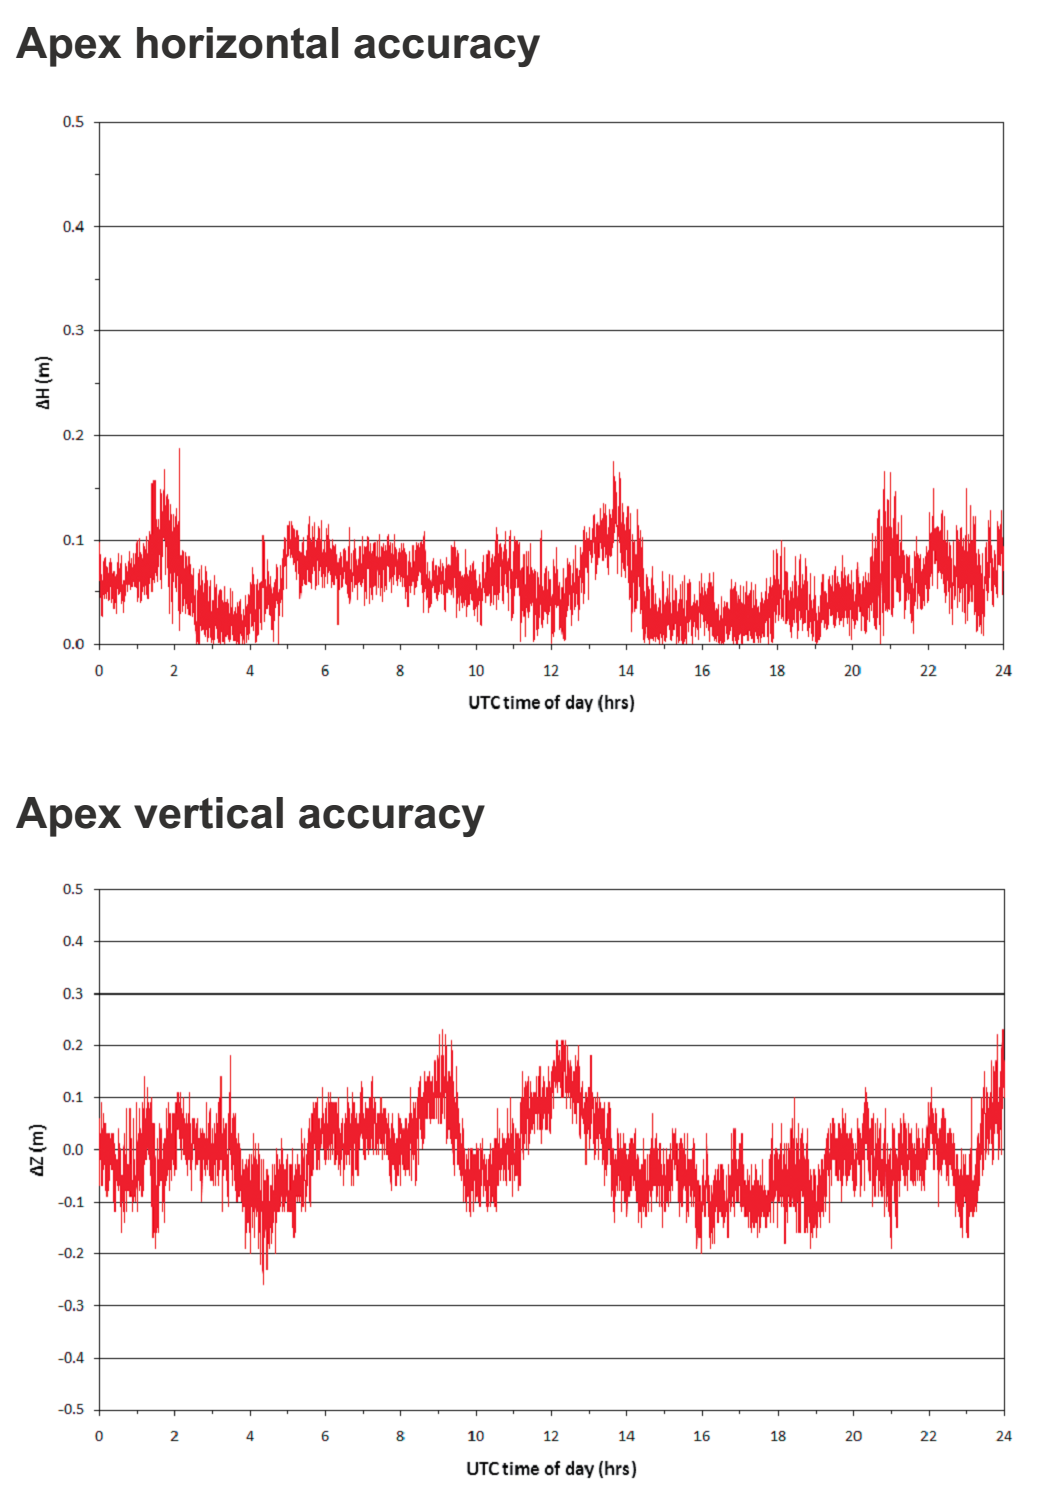
\includegraphics[height=0.8\textheight]{pic/Apex.png}
		\caption{VERIPOS Apex solution at a monitor site in Aberdeen.}
	\end{figure}
	
\end{frame}






\section{Processing details}

\begin{frame}{Live demo}
	
Live demo...
	
	
	
\end{frame}


\begin{frame}{Practice}
	
	\begin{itemize}
		\item DL5 will be restarted at 12:00 in order to converge properly.
		\item You will start collecting RTK data after 14:00. 
		\item VERIPOS Ultra uses a different technique. Instead of providing DGPS corrections for
		distinct reference stations it uses global orbit \& clock correction message.
	\end{itemize}
	

	
\end{frame}


\begin{frame}{NGB5}
	\begin{table}
		\centering
		\begin{minipage}[t]{\textwidth}%
			\resizebox{\columnwidth}{!}{%
				\begin{tabular}{lccccc} %{l|c|c|c|c}
				\toprule %\rowcolor{lightgray}
				 Point & Frame & Lat[deg]  & Long[deg]  & EllHt[m] & Notes\tabularnewline
				\midrule
				NGB5 & ERF97 & 52 57 07.05318 & 01 11 01.44897 W & 91.2065 & at point\\
				NGB5 & ERF97 & 52 57 07.05318 & 01 11 01.44897 W & 91.3865 & at ARP\footnote{Antenna heigh = 0.18m.}\\
				NGB5 & ERF97 & 52 57 07.05318 & 01 11 01.44897 W & 91.4280 & at antenna PCO\footnote{Ionsphere free antenna offset is $2.545L_1-1.545L_2$ so\\ $2.545*55.3-1.545*64.2=41.5mm$.}\\
				\textbf{NGB5} & ITRF2008 & \textbf{52 57 7.070524} & \textbf{01 11 1.427085} W & \textbf{91.480} & at antenna PCO\footnote{Converted from ETRF97 to ITRFT2008 at epoch 2015-12-04.} \\
				\bottomrule
			\end{tabular}%
			}
			\caption{Coordinates of NGB5}
		\end{minipage}
	\end{table}
	
\end{frame}




\begin{frame}{Taking things forward}
\begin{Large} %make text large
	Any Questions?
\end{Large}
\end{frame}

\end{document}
